% generated by build_assets.py from the recorded PDF and caption; do not edit
\begin{figure}[tbp]
\centering
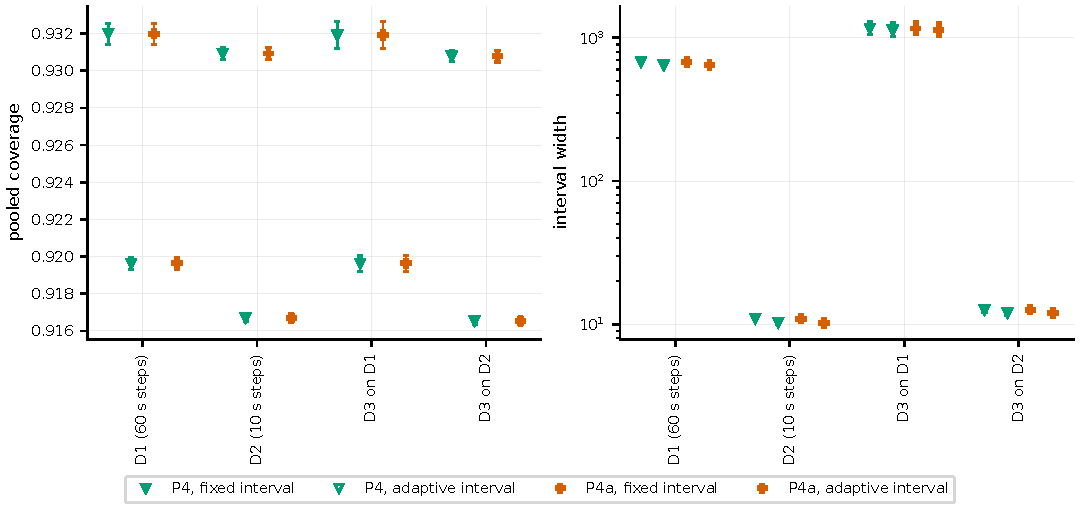
\includegraphics[width=\linewidth]{assets/figures/fa14_conformal_logging.pdf}
\caption{FA14. Conformal interval logging (RV4): pooled coverage (left) and interval width (right, log scale) of the fixed and the adaptive interval, for P4 and P4a, per dataset (widths are not comparable across datasets). Filled markers: fixed interval; open: adaptive. Mean with its 95\% BCa interval over events (9999 resamples, master seed 42). The table holds pooled values, so there is no time axis; the adaptive level (alpha), the point error and the trigger counts are in the table and not drawn. Events per dataset: D1 60; D2 60; D1\_D3 40; D2\_D3 40. Source: tables/rv4\_logging.csv.}\label{fig:fa14_conformal_logging}
\end{figure}
